\chapter{Methodology}

\section{\label{data_collection}Data Collection}

    When mining Github and Stack Overflow, a natural starting point is to use GHTorrent \cite{gousios2013ghtorent} and SOTorrent \cite{baltes2018sotorrent} as data sources.
    \subsection{Stack Overflow data}
        SOTorrent\footnote{\label{SOTorrent}\url{https://empirical-software.engineering/projects/sotorrent/}} is an open data set based on periodic, official Stack Overflow data dumps. SOTorrent was built for the purposes of mining and analyzing the evolution of Stack Overflow posts. A new version of this data set based on the latest Stack Overflow data dump is released every 3 months. Each version of the SOTorrent datas set can be downloaded from Zenodo\footnote{\label{SOTorrent_Zenodo} \url{https://zenodo.org/record/2273117}}. The latest versions of the SOTorrent data set are also available online, and can be queried through Google BigQuery\footnote{\label{BigQuery} \url{https://bigquery.cloud.google.com/dataset/sotorrent-org:2018_12_09}}.
        
        When downloading the SOTorrent data set, the version from \textit{December 9th 2018} was used, as it was the latest version available at the start of the project. The SOTorrent data set has its files organized into tables. Not all tables were downloaded, as certain tables related to post evolution (e.g. PostHistory, PostVersion tables) were deemed to be unrelated to the expertise learning task. The tables downloaded included Users, Posts, PostLinks, PostType, PostReferenceGH, Comments, CommentUrl, GHMatches, Tags, Badges and Votes, totaling 29 GB of compressed raw data. After downloading and un-compressing all relevant data files, the data set contained just shy of 100 GB of data.
        
    \subsection{Github data}
        GHTorrent\footnote{\label{GHTOrrent}\url{http://ghtorrent.org/}} is also an open data set, which mirrors the data offered through the Github REST API\footnote{\url{https://developer.github.com/}}. GHTorrent has been collecting data from all public projects available on Github and releases a new version of MySQL data dumps every month, while it also offers daily data dumps through MongoDB. Each version of MySQL data can be downloaded from GHTorrent\footnote{\label{GH_dowload}\url{http://ghtorrent.org/downloads.html}}. GHTorrent data can also be looked at and queried online, as it is available as a DBLite web interface\footnote{\label{GH_query}\url{http://ghtorrent.org/dblite/}}. 
            
        When downloading the GHTorrent data set, the version from \textit{March 1st 2019} was used, as it was the latest version available at the time of download. The data set has its files organized into large tables stored in compressed CSV files, totaling 96557 MB of compressed data. All files were downloaded and uncompressed which resulted in 21 raw data tables totaling over 400 GB of data.

\section{Data Storage}

    \subsection{Database Setup and Data Import}
        
        A MySQL database was the obvious choice of database, as both data sources come with SQL scripts performing table creations, data imports and general database manipulations\footnote{\label{SO_sql} \url{https://github.com/sotorrent/db-scripts/tree/master/sotorrent}} \footnote{\label{GH_sql} \url{https://github.com/gousiosg/github-mirror/tree/master/sql}}. Managing disk space during the data import phase represented a challenge, as the raw, uncompressed data files totaled up to over 500 GB. Importing of the data into the database was not achieved all at once, but rather through several iterations of uncompressing only a few data files. After a file was uncompressed and the table was successfully imported into the database, its raw CSV or XML file was deleted to free up disk space. 
        
        During the data import phase it was discovered that using \textit{MyISAM} over \textit{InnoDB} as the database engine is more favorable, since there was a significant execution time difference between the two database engines when importing large amounts of data into the MySQL database. \textit{MyISAM} database engine does not support foreign keys constraints, while it supports table-level locking. On the other hand \textit{InnoDB} supports foreign key constraints and row-level locking. \textit{MyISAM} is preferred when performing tasks that require fast import and querying speed, while \textit{InnoDB} being the default database engine for MySQL is more optimal for regular operations. For this particular reason all of the large raw data files were imported into the database using the \textit{MyISAM} database engine. After all necessary database manipulations have been performed, the database engine was changed back to the default engine, \textit{InnoDB}, to allow foreign key constraints to be enforced. 
     
        \todo{Add table contains descriptions for each relation's content}
      
        \begin{figure}[!ht]
          \centering
          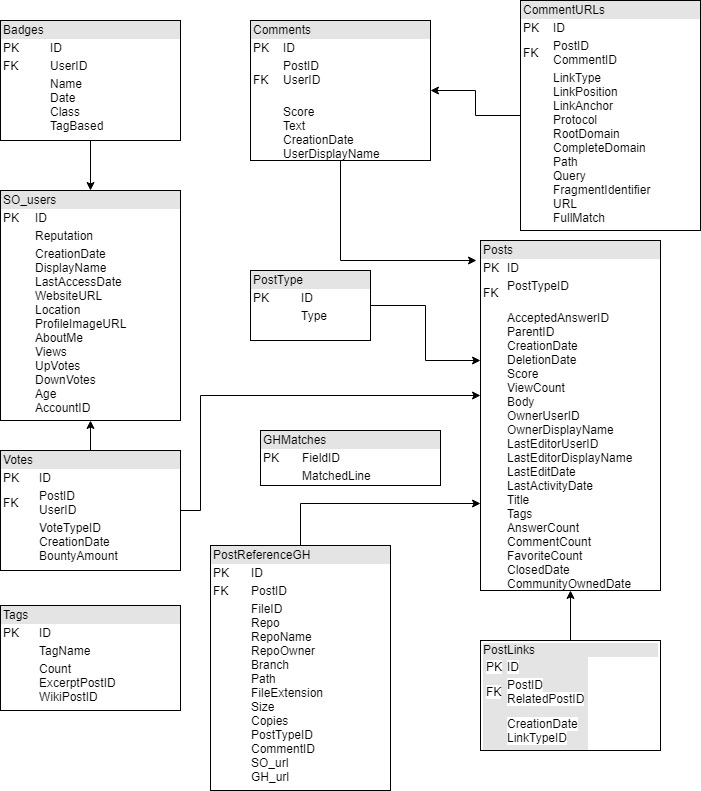
\includegraphics[width=0.9\textwidth]{SO_DB_schema.jpg}\\
          %\caption{Redesigned database schema for the downloaded Stack Overflow data.}
          \label{fig:so_schema}
        \end{figure}
        
   
        \todo{Re-do this image}
        \begin{figure}[!ht]
          \centering
          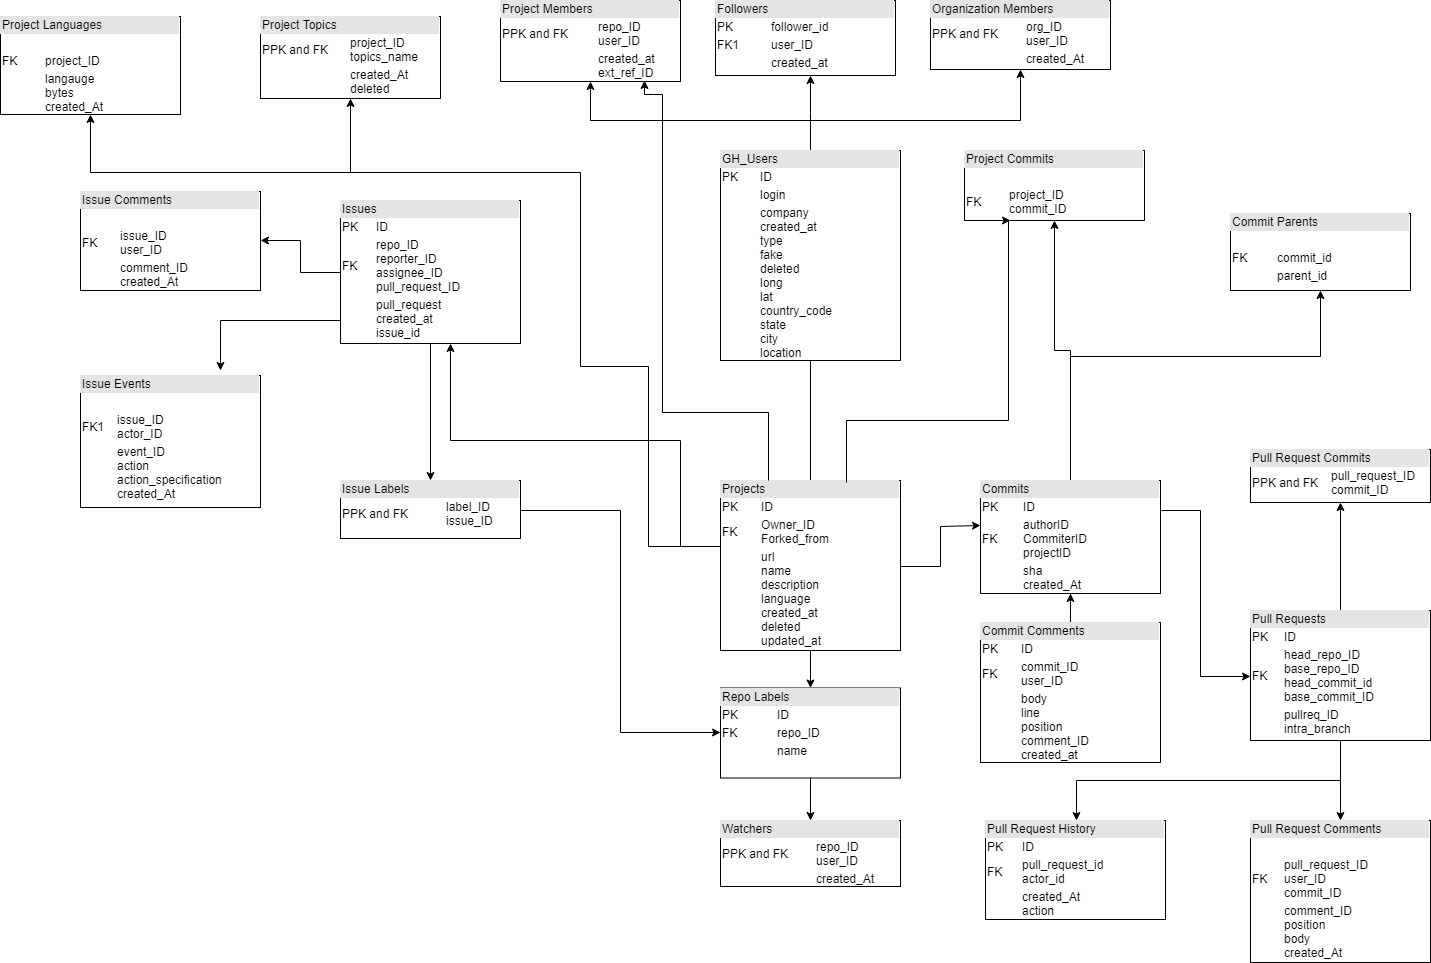
\includegraphics[width=\textwidth]{GH_DB_schema.jpg}\\
          %\caption{Redesigned database schema for the downloaded Github data.}
          \label{fig:gh_schema}
        \end{figure}
        
        Figure \ref{fig:so_schema} and \ref{fig:gh_schema} show the database schema and all attributes within each table of the SOTorrent and respectively the GHTorrent data set. All tables from GHTorrent are shown in figure \ref{fig:gh_schema}, while only the relevant tables from SOTorrent are shown in figure \ref{fig:so_schema}. 


    \subsection{Linking together GHTorrent and SOTorrent}\label{Linking_SO_GH}
    
        In order to perform cross platform analysis of Github and StackOverflow, the linking of GHTorrent and SOTorrent datasets is needed. This task requires identifying the same user's accounts on both platforms. Looking at relevant literature on this this problem, one can identify the task of \textit{identity merging}, which consists of identifying the same person in two or more different environments. Vasilescu et al. \cite{vasilescu2013stackoverflow} researched this problem rigorously and after careful consideration of limiting the number of false positives they made use of email addresses. In 2013, at the time of publishing their work, email addresses were present in the Github dataset, while in the StackOverflow dataset email addresses were hidden, but their MD5 hashes were available. Vasilescu et al. \cite{vasilescu2013stackoverflow} decided to ``merge (i.e., link) a GitHub and a Stack Overflow user if the computed MD5 hash [of the email in Github] is identical to the MD5 email hash [of Stack Overflow users]". This resulted in 93,771 GitHub users being linked to StackOverflow. Vasilescu et al. \cite{vasilescu2013stackoverflow} further investigated, and came to the conclusion that out of 93,771 linked users only 46,967 users were active at the time. The linked data set alongside a replication package has been made public by the authors of the paper\footnote{\label{bodgan_dataset}\url{https://www.win.tue.nl/mdse/stackoverflow/}}. This data set has been used multiples times to analyze the interaction of Github and Stack Overflow data \cite{badashian2014involvement} and \cite{lee2017github}, thus it became the backbone of the data sampling process behind linking together Github and Stack Overflow users.  

        There was one major problem with using Vasilescu et al. \cite{vasilescu2013stackoverflow}'s data set. The replication package contained a data set linking Github email addresses to Stack Overflow user IDs, without fully mapping Github user IDs to Stack Overflow user IDs, therefore the mapping of Github email addresses to user IDs was needed. This mapping was possible when Vasilescu et al. \cite{vasilescu2013stackoverflow} published their work, but after March 2016 GHTorrent was not allowed to store email addresses in their open data sets, as it violated GDPR compliances. The solution to this problem was to download the \textit{User} table data from GHTorrent's last available version that still contains email addresses of Github users in the data set. This older version of GHTorrent is dated \textit{February 1st 2016}, and it was downloaded, then imported into the MySQL database. A manual check was performed on matching user IDs and login names between the \textit{User} table's March 2019 and February 2016 versions. This manual check made sure that the user IDs from both versions of the table are referring to the same login name. If this was not the case, the user was dropped from the data set, due to inconsistency of the two versions of table. This manual check assured consistency in the data linkage between Stack Overflow and Github users, but resulted in the removal of over 10,000 users from the original 93,771 users linked. The final data set contains 83,550 user accounts being linked between the two platforms, offering a unique Github user ID to Stack Overflow user ID mapping. It can be speculated that removed users either deleted or changed the login name of their Github account between 2016 and 2019, thus causing the inconsistency in the two versions of the \textit{User} table.
        
    \subsection{Discarding Unlinked Data}
       As mentioned in section \ref{data_collection}, the total size of the GHTorrent data set was over 400 GB of data, while SOTorrent contained close to 100 GB of data. In order to make data querying and processing more efficient, the reduction the full data set was desired. In order to perform analysis only on the linkage between Github and Stack Overflow, only successfully linked data is needed. Filtering out unlinked data was done by iterating through each existing table in the database and keeping only the observations that are connected or related to users with a user ID present in the list of 83,550 unique user IDs linked. Discarding unlinked data reduced the size of the data set and allowed only linked data to be analyzed. This process reduced the size of the MySQL database from over 500 GB of data to 122 GB.
        
\section{Data Aggregation} 
    The end goal of the analysis on Stack Overflow and Github data was to create topic models capable of deciphering the hidden patterns of underlying topics that represent a user's activity on a platform. Tian et al. \cite{tian2013predicting} modeled user topical interest and expertise by building LDA models on user activity (user profile) data. The authors have showed that a Stack Overflow user's expertise can be extracted using a topic model applied over a set of textual documents consisting of the user's activity on the platform collected into a user profile.

    In order to perform cross platform analysis of Github and Stack Overflow users' expertise, the modeling of their expertise through LDA models is needed. LDA topic models are fit on a set of documents. In order to fit LDA models on Github and StackOverflow user data, one needs to define what a document consists of, and how to extract a user's profile from a platform such as Github or Stack Overflow.  
    
    \subsection{Extracting Stack Overflow User Profiles\label{SO_userProfileExtraction}}
        When deciding how to create documents for the LDA topic model, the simplest approach was to define a document as a user profile. Each user present in the data set of 83,550 linked users described in section \ref{Linking_SO_GH} has one document (user profile) describing their activity on Stack Overflow. This document contains all of their activity on the platform. Extracting a user's activity (user profile) from all the public data stored about a user started by inspecting each table of the SOTorrent database schema \ref{fig:so_schema} for attributes that contain relevant and meaningful textual information about a user. The relevant textual attributes included into Stack Overflow user profiles were badge names obtained by a user, the description on the profile page's about me section, questions posted by a user, answers given by a user, titles and tags of posts that a user participated in, and comments made by a user to any post.
          
        \begin{table}[!htbp]
            \centering
            %\caption{Sample table. With an extra long caption to test how captions will wrap.}
            \label{tab:SO_userProfileExtraction}
            \vspace{6pt} % Required to get proper spacing between caption and table
            \begin{tabular}{|p{3cm}|p{3cm}|p{8cm}|}
               \toprule
               \textbf{Name} & \textbf{Attribute(s)} & \textbf{Derivation} \\
               \toprule
                Badges & Badges.Name & Concatenation of list of badges obtained by the user \\
                About Me & Users.AboutMe & Stack Overflow user profile's about me description \\
                Post Answer & Posts.Body, AcceptedAnswerId & Take a user's each answer and concatenate it with the question that it is related to  \\
                Post Question & Posts.Body & Take a user's each question and concatenate it with the accepted answer it is related to  \\
                Title and Tags for Questions & Posts.Tags, Posts.Title & Concatenate the post tags and title for each question that the user asked \\
                Title and Tags for Answers & Posts.Title, Posts.Tags & Concatenate the post tags and title for each answer that the user provided \\
                Comments & Comments.Text, Posts.Body, Posts.Title & Take a user's each comment and concatenate it to the post (question or answer) it is related to \\
               \bottomrule
            \end{tabular}
        \end{table}  
        
       A detailed description on how data was manipulated for these user profile attributes can be found in table \ref{tab:SO_userProfileExtraction}.
    
        % to do: explain the logic behind joining Q + A (for context)
        % to do: explain that all this will get concatenated into 1 giant string
        
    \subsection{Extracting Github User Profiles\label{GH_userProfileExtraction}}
        Each user present in the data set of 83,550 linked users described in section \ref{Linking_SO_GH} has one document (user profile) describing their activity on Github. Extracting a user profile was done my inspecting each table of the GHTorrent database schema \ref{fig:gh_schema} for attributes that contain relevant textual information about a user. The textual attributes selected to be part of the user profile data include the names, labels, languages used and description of each repository that a user owns, also their commit and pull request comments posted on Github. 
        
        \begin{table}[!htbp]
            \centering
            %\caption{Sample table. With an extra long caption to test how captions will wrap.}
            \label{tab:GH_userProfileExtraction}
            \vspace{6pt} % Required to get proper spacing between caption and table
            \begin{tabular}{|p{3cm}|p{3cm}|p{8cm}|}
               \toprule
               \textbf{Name} & \textbf{Attribute(s)} & \textbf{Derivation} \\
               \toprule
                Project Name, Description \& Metadata & Projects.(name, description, language), Repo-Labels.name & Take each user's each project and concatenate the repository's name, description, languages used and repository labels it contains\\  
                Commit-Comments & Commit-Comments.body & Concatenate a user's list of commit comments \\
                Code-review Comments & Pull-Request-Comments.body & Concatenate a user's list of code review (pull request) comments \\
               \bottomrule
            \end{tabular}
        \end{table}
        
        A detailed description on how data was manipulated for these user profile attributes can be found in table \ref{tab:GH_userProfileExtraction}.
        
        % to do: explain the logic behind selecting these attributes
        % to do: explain that all this will get concatenated into 1 giant string
        
    \subsection{Creating Time Based User Profiles}
        After defining how to extract user profiles from both Stack Overflow and Github, it is worth factoring in a \textit{timeline} into the user profile. The simplest approach would be to model recent and past activity of users by splitting their activity into before and after a specific date. Being able to model past and recent user profile data separately creates opportunities for comparison analyses to be done on the evolution of expertise of Github and Stack Overflow users. A decision was made to define recent activity as the activity performed by a user in the last 3 years. 2019 being the year that this analysis has taken part, the split between past and recent activity was created by any user profile data being dated before or after \textit{January 1st 2016}.
        
        % talk about full, past, and recent versions of the dataset

\section{Data Cleaning}
Textual data on Stack Overflow and Github contains a large variety of software engineering related domain specific wording mixed with source code. Stack Overflow posts contain rich software artifacts such as code snippets, text blocks explaining problems and solutions using text and source code, comments which can be associated with a question or an answer, and hyperlinks to references such as API documentation or an academic paper explaining an answer. In their study of Github data, Liao et al. \cite{liao2019status} mentions that developers on Github ``talk about project bugs, enhancements, and tasks in issue discussions". The authors stated that a text corpus built on Github data will most likely contain ``plenty of code, warnings, messages, and technical terminology in addition to more general natural language [...] which allow for easy detection of status and/or relevant expertise".

One can conclude that textual data on both Github and Stack Overflow captures a variety of aspects of software development, but its technical terminologies, mix of text and source code makes it difficult to extract the proper textual data to be analyzed. When performing text pre-processing on both sources of data, one needs to find the right balance between more than a dozen pre-processing techniques in order to clean up the data just the right way, without removing software engineering domain specific words and damaging the contextual details of software artifacts. Deciding on a precise set of techniques for the pre-processing routine was a challenging task, thus extensive research was done on what text pre-processing techniques were previously used when analyzing Github and Stack Overflow data.

Tian et al. \cite{tian2013predicting} pre-processed textual data by performing tokenization, stop-word removal and stemming. They also split function names from cleaned up source code related keywords in the text processing phase.

Campbell et al. \cite{campbell2015latent} mentions in a book chapter on extracting topics from software engineering data that generally those who use LDA apply the following pre-processing steps: ``loading text, mapping text into final textual representation, [perform] lexical analysis of the text, optionally removing stop words, optionally stemming, building a vocabulary, optionally removing uncommon or very common words and mapping each text document into a word-bag".

Treude and Wagner \cite{treude2019predicting} have performed similar, but separate pre-processing routines on StackOverflow and Github data. Their Stack Overflow data cleaning routine consisted of removing line breaks, code blocks, all HTML tags, replacing HTML symbols and strings indicating special characters with their corresponding character, and replacing sequences of whitespace with a single space. Their Github pre-processing routine is the same as the above Stack Overflow data cleaning routine, with a few extra steps, such as removing vertical and horizontal lines, code comments, characters denoting sections headers, characters that indicate formatting or links. 

Efstathiou et al. \cite{efstathiou2018word} converted text from Stack Overflow into lowercase, removed code snippets and HTML tags, then performed a ``conservative punctuation removal, keeping symbols that often appear in programming commands, such as ‘+’ and ‘\#’ which are essential for differentiating ‘C’, ‘C++’, and ‘C\#’ from one another."

Boyd-Graber et al. \cite{boyd2014care}'s book chapter recommends HTML symbol and  stopword removal, then normalizing strings by converting to lower case and applying any kind of stemming algorithm, then apply tokenization and any kind of phrase detection algorithm as the proper pre-processing routine before fitting topic models on textual data.

Liao et al. \cite{liao2019status} analyzed issue discussions on Github, and in their pre-processing steps they filtered out code-specific language, which was enclosed in HTML tags. The authors then removed short posts contained less than five tokens and distinguished between data generated by developers who never committed code to a project, and those who did. 

Based on the above data cleaning routines used when working with software engineering domanin specific textual data, a user level and a corpus level pre-processing routine was developed. The user level pre-processing routine is executed on each user's aggregated textual data individually during the user profile extraction processing described in sections \ref{SO_userProfileExtraction} and \ref{GH_userProfileExtraction}. The user level routine involved the removal of html links, symbols and tags, proceeded by stop-word, mentions (using @) and multiple white space removal. Finally, a tokenization technique is applied, then individual tokens consisting of only numbers or punctuation with no words present in the token are removed. This data processing routine is executed on the already aggregated (concatenated) data obtained using the description in sections \ref{SO_userProfileExtraction} and \ref{GH_userProfileExtraction}.

The corpus level pre-processing routine is executed on each individual text corpus (GH-past, GH-recent, GH-full, SO-past, SO-recent and SO-full) before the model fitting, but after the data aggregation process. The corpus level pre-processing includes tokenization, standardization of tokens, frequent phrase detection, then removing tokens that include only numbers and punctuation(if any). A subset of symbols and punctuations were also removed, keeping symbols such as ‘+’, ‘\_’, ‘.’ and ‘\#’, which often appear in programming contexts. Finally, rare and very common tokens are removed by filter out tokens that occur in less than 10 documents, or more than 50\% of the documents. In this context standardization of tokens means re-writting common tokens spelled multiple ways as a unique token. Examples of such common tokens include ‘node.js’, ‘node-js’, ‘node\_js’ for ‘nodejs’; ‘angular.js’, ‘angular-js’, ‘angular\_js’ for ‘angularjs’; or ‘js’ for ‘javascript’, and many more. A list of the most frequent phrases detected in the GH-full and SO-full data sets can be found in appendix \ref{frequentExpressions}. These common phrases used in the software engineering domain have totally different meaning as a phrase(bigram), thus they have been re-written as a single word (unigram), using a ‘\_’ character connecting the phrases. As a final note on data cleaning, both user and corpus level pre-processing routines were designed based on common best practises of previous data cleaning routines (\cite{tian2013predicting}, \cite{campbell2015latent}, \cite{treude2019predicting}, \cite{efstathiou2018word}, \cite{boyd2014care}, \cite{liao2019status}).

\section{Topic Modeling}
% why are we using topic models ?
The inspiration to use topic modeling to learn cross-platform developer expertise came from Tian et al. \cite{tian2013predicting}'s work. The authors used topic models to predict the best answerer for a new question on Stack Overflow. Their approach learnt user topical expertise and interest levels by profiling each user's previous activity and reputation on Stack Overflow. In software engineering applications when working with large collections of textual data the most popular topic modeling technique to use is Latent Dirichlet Allocation (LDA) \cite{campbell2015latent}. 

In their book chapter titled \textit{Latent Dirichlet Allocation: Extracting Topics from Software Engineering Data}, Campbell et al. \cite{campbell2015latent} is stating that ``LDA can be used to summarize, cluster, link, and preprocess large collections of data because it produces a weighted list of topics for every document in a collection dependent on the properties of the whole. These lists can then be compared, counted, clustered, paired, or fed into more advanced algorithms. Furthermore, each topic is comprised of a weighted list of words which can be used in summaries."

LDA models have been previously used to learn semantic similarity between user profiles, posts (\cite{tian2013predicting}) and even source codes (\cite{arwan2015source}) on Stack Overflow. The proposed novel approach is creating a cross-platform developer expertise extraction task consisting of topical expertise learnt from topic analysis on user profiles extracted through mining public software repository platforms like Stack Overflow and Github. Campbell et al. \cite{campbell2015latent}'s explanation on the use of LDA models shows that extracting such expertise is possible by providing a summary or ranking of the the weighted list of topic words for each topic that the user is present in or belongs to. 
    
    \subsection{Model Setup}
        % TO DO: mention the data sets that we fit LDA on, having diff. LDA models
    
        As mentioned in section \ref{SO_userProfileExtraction} and \ref{GH_userProfileExtraction}, before fitting an LDA model, a document was defined as a user profile. There are 83,550 linked users in the data set, each user having only one document (user profile) describing their activity, thus when fitting an LDA model, there are always 83,550 documents to be fitted on. 
        
        %% Creating SO-full and GH-full after inactive user issues
        
    
    \subsection{Hyper-Parameter Optimization}
    When analyzing the misuse of LDA common practises Agrawal et al. \cite{agrawal2018wrong} concluded that ``using the default settings of LDA for software engineering data can lead to systematic errors due to topic modeling instability". For instance, most LDA implementations recommend and use by default a fixed normalized asymmetric prior of $1.0 / topic-number$ for the $\alpha$ parameter, and a fixed prior of $0.01$ or $0.1$ for the $\beta$ parameter. In their study of good configurations of LDA models for GitHub and Stack Overflow data Treude and Wagner \cite{treude2019predicting} confirmed the findings of \cite{agrawal2018wrong} by concluding that ``popular rules of thumb for topic modelling parameter configuration are not applicable to textual corpora from GitHub and Stack Overflow. These corpora have different characteristics and require different configurations to achieve good model fit." Furthermore, Agrawal et al. \cite{agrawal2018wrong} clarifies by stating that ``any study that shows the topics learned from LDA, and uses them to make a particular conclusion, needs to first tune LDA,  [since] topics learned from untuned LDA are unstable, [but] after tuning, stability can be greatly increased." The authors also note that reusing hyper-parameter tunings suggested by other researchers from other data sets is not a reliable option, as the best LDA tunings differ from data set to data set, and LDA models always need to be re-tuned for all new data.
    
    To address these concerns of LDA misuse, the models fitted in this project use 400 iterations through the corpus when inferring the topic distribution of a corpus (instead of default 50 iterations). This should assure model's stability, as model convergence is checked before finishing the fitting process. For the random state of the model training initialization a fixed seed is used to promote reproducibility. 
    
    In terms of the $\alpha$ and $\beta$, hyper-parameter optimization is performed by combining the best practises of Bangash et al. \cite{bangash2019developers} and Treude and Wagner \cite{treude2019predicting}' work on finding the right hyper-paramters. Hoffman et al. \cite{hoffman2010online}'s implementation of \textit{Online learning for LDA models} is used to learn an asymmetric prior from the data for both $\alpha$ and $\beta$  hyper-parameters.
    
    %% deciding on k

    
    %% These results also ask us to revisit the previous case studies which have used LDA using “off-the-shelf” parameters to rerun by tuning these parameters using automated tools like LDADE.
    
    \subsection{Evaluation of model}
    
    \section{Expertise survey}
        \subsection{Survey setup}
        %% task, sampling, who did it
        \subsection{Annotations Cleaning}
        \subsection{Limitations}
        % aggregating the data, (union and intersect)
        
\section{Data Analysis and Algorithm Design}
    %%for each technique
        %% what it is, where do you use it
    
    \subsection{Extracting/ Determining Expertise}
    
        %% mean_BLEU_score, mean_Jaccard_sim, Mean_Cos_sim
        \subsubsection{Topic Distribution based Expertise}
        %%% (mention Lda2vec and ETM as alternatives)
        
        \subsubsection{User and Topic Embeddings}
        %%% Avg and Max LDA Emb
        %%% Avg and Max word2vec Emb
        
        %%% k-means, then thresholding
        
    \subsection{Cross-platform expertise}
    %% RQ2 - quantitative diff - distr. of overlap or Jaccard sim.
    \subsection{Cross-platform Knowledge Transfer}
    %% RQ3 - most frequent words used in both platforms
    \subsection{Expertise Evolution}
%% RQ4 - changed ratio or Jaccard dist.

\section{Software Tools Used}



    
